\pgfplotsset{
    standard/.style={%Axis format configuration
        axis x line=middle,
        axis y line=middle,
        enlarge x limits=0.15,
        enlarge y limits=0.15,
        every axis x label/.style={at={(current axis.right of origin)},anchor=north west},
        every axis y label/.style={at={(current axis.above origin)},anchor=north east},
        every axis plot post/.style={mark options={fill=white}}
        }
  }
  \begin{figure}[hb!]
    \centering
    \subfloat[ ]   { %Unit step squence
      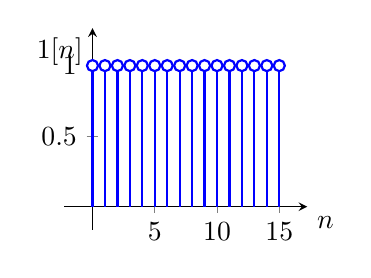
\begin{tikzpicture}
        \begin{axis}[%
          scale=0.45,
          standard,
          domain = 0:15,
          samples = 16,
          xlabel={\(n\)},
          ylabel={\(1[n]\)},
          ymin=0,
          ymax=1.1]
          \addplot+[ycomb,blue,thick] {1};
        \end{axis}
      \end{tikzpicture}
    }
    \subfloat[ ]   { %Sampled sine squence
      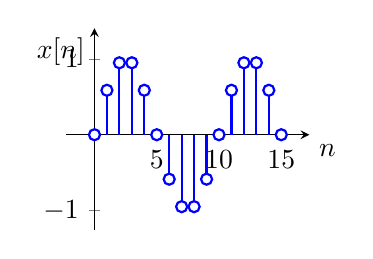
\begin{tikzpicture}
         \begin{axis}[%
            scale=0.45,
            standard,
            domain = 0:15,
            samples = 16,
            xlabel={$n$},
            ylabel={$x[n]$},
            ymax=1.1]
            \addplot+[ycomb,blue,thick] {sin(5*180*x/25)};
         \end{axis}
      \end{tikzpicture}
    }
    \caption[Posloupnost jednotkového a obecného signálu]{Posloupnost jednotkového skoku $1[n]$
             a signálu $x[n]$}
    \label{SAS:fig_odezva4}    
  \end{figure}
